\section{Ejercicio 2}

Peso asignado: X.

\subsection{Problema}

Se tiene una lista de direcciones de correo electrónico y un apodo por cada
uno. Los apodos son siempre prefijos de su correspondiente dirección. El
problema consiste en obtener el mínimo valor de T que cumpla que para cada
dirección que se pase junto con su prefijo, existen a lo sumo T direcciones
que comparten ese prefijo.

Esto en otras palabras, se debe obtener la cantidad de veces que se repite el
prefijo que se comparte la mayor cantidad de veces.

\subsection{Resolución}

\subsubsection{Explicación y correctitud}

Se debe encontrar cuántas veces se comparte el prefijo más repetido. Para ello
podría simplemente tomar cada uno de los prefijos, comprobar si es prefijo de
cada dirección, y de el resultado tomar el que más veces se comparte. El
problema es que ese algoritmo no cumpliría la complejidad requerida. Así que
para solucionarlo se utiliza una estructura de árbol con invariante de Trie
en donde se almacenan las direcciones.

\begin{figure}[ht]
	\caption{Trie de direcciones}
	\label{ej2:trie}
	\centering
	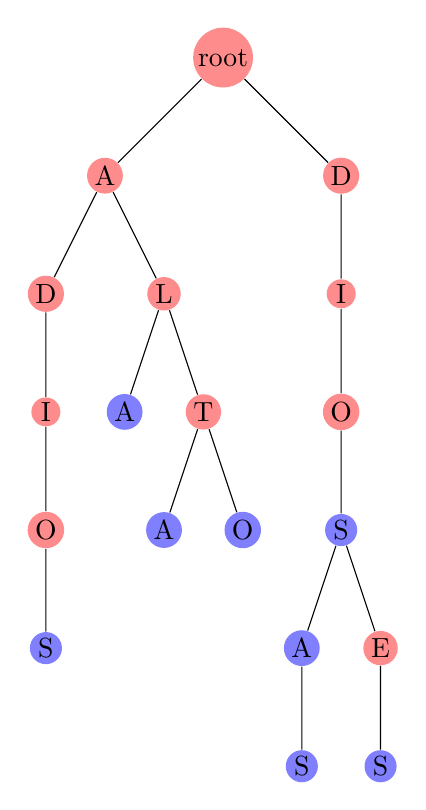
\begin{tikzpicture}
	[sibling distance=3cm,
	level 2/.style={sibling distance=1.5cm},
	level 3/.style={sibling distance=1cm},
	every node/.style={fill=red!45,circle,inner sep=1pt}]
	\node {root} [grow=down]
	child { node {A}
		child { node {D}
			child { node {I}
				child { node {O}
					child { node [fill=blue!50] {S} }
				}
			}
		}
		child { node {L}
			child { node [fill=blue!50] {A} }
			child { node {T}
				child { node [fill=blue!50] {A} }
				child { node [fill=blue!50] {O} }
			}
		}
	}
	child { node {D}
		child { node {I}
			child { node {O}
				child { node [fill=blue!50] {S}
					child { node [fill=blue!50] {A}
						child { node [fill=blue!50] {S} }
					}
					child { node {E}
						child { node [fill=blue!50] {S} }
					}
				}
			}
		}
	};
	\end{tikzpicture}
\end{figure}

Puede observarse en la Figura \ref{ej2:trie} que algunos nodos del árbol están
marcados en color azul. Estos nodos representan el final de una palabra. De
esta forma pueden almacenarse palabras que sean prefijos de otras.

Lo que se hace entonces es almacenar las direcciones en dicho árbol, pero a
su vez se almacena la cantidad de veces que una letra es parte del mismo
prefijo. Por ejemplo, si se agregan ``hola'' y ``hotel'' las letras `h' y `o'
quedarían 2 veces repetidas mientras que el resto sólo una. El ejemplo se
ilustra en la Figura \ref{ej2:trie_rep}

\begin{figure}[ht]
	\caption{Trie de direcciones con repeticiones}
	\label{ej2:trie_rep}
	\centering
	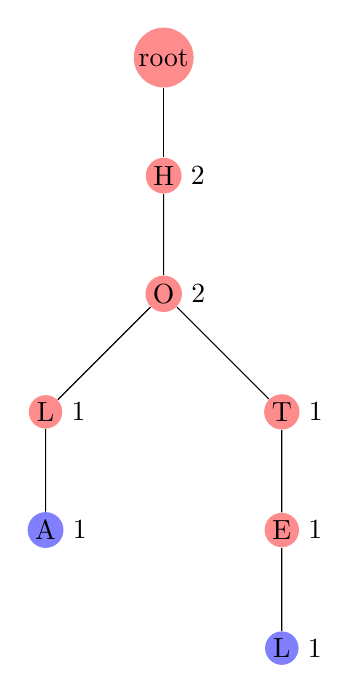
\begin{tikzpicture}
	[sibling distance=3cm,
	every node/.style={fill=red!45,circle,inner sep=1pt}]
	\node {root} [grow=down]
	child { node [label=right:2] {H}
		child { node [label=right:2] {O}
			child { node [label=right:1] {L}
				child { node [label=right:1,fill=blue!50] {A}}
			}
			child { node [label=right:1] {T}
				child { node [label=right:1] {E}
					child { node [label=right:1,fill=blue!50] {L} }
				}
			}
		}
	};
	\end{tikzpicture}
\end{figure}

Los prefijos se almacenan en una lista de strings. Una vez hecho esto, se
recorre la lista y para cada prefijo se lo busca en el Trie. Dicha búsqueda
devuelve la cantidad de apariciones del prefijo, consultando el numero de
apariciones del último nodo. De estas búsquedas se toma la de mayor valor y
ese es el resultado que se retorna. Por lo tanto el valor obtenido representa
la cantidad de veces que se comparte el prefijo con mayor número de
repeticiones.

El Trie esta implementado através de una clase que tiene 3 propiedades:

\begin{itemize}
\item Un arreglo de punteros a Trie de 256 elementos llamado \textit{hijos}
\item Un bool que indica si el nodo representa el final de una entrada llamado
\textit{final}
\item Un int que indica la cantidad de veces que la letra es prefijo de alguna
palabra llamado \textit{apariciones}
\end{itemize}

Al insertar una palabra en el árbol lo que se hace es recorrer recursivamente
el string y incrementando la posición del elemento a tener en cuenta.
Empezando por la raiz del árbol (que representa el caracter vacío) se examina
el primer caracter del string. Su codigo ASCII corresponde a uno de los 256
elementos del arreglo de punteros a Trie que se tiene. El procedimiento es el
siguiente:

\begin{enumerate}
\item Se incrementa la cantidad de apariciones
\item Si es el final del string se setea el bool en true y se termina la
ejecución
\item Si el puntero correspondiente a la letra en cuestión es nulo, se crea
una nueva instancia de Trie llamando a su constructor, el cual setea todos los
hijos en NULL, establece la cantidad de apariciones en 1 y por último pregunta
si es el final de la cadena. De serlo se pone final en verdadero. De lo
contrario se llama recursivamente al constructor pasándo el mismo string como
parámetro pero incrementando en 1 la posición que debe examinarse
\item Por último, llegado a este punto significa que no es la última posición
de la cadena y que existe un nodo para la letra actual. En este caso se llama
recursivamente a la insercion incrementando en 1 la posición del caracter en
cuestión
\end{enumerate}

Este proceso deja una estructura en la cual cada caracter tiene asociado un
número el cual fue incrementado una vez cada vez que la inserción de una
cadena recorrió ese nodo. Esto significa que consultar dicho número dice
qué cantidad de veces se insertó un prefijo que llega hasta ese caracter.
Por lo tanto haciendo la búsqueda para cada prefijo se obtiene la cantidad de
veces que este aparece.

\subsubsection{Pseudocódigo}

A continuación se expone un pseudocódigo de las funciones de inserción y
búsqueda del Trie.

~

\begin{algorithm}[H]
	\caption{insertar}
	\Input{$String\&$ $prefijo$, $Entero$ $pos$}

	$apariciones$++ \;
	\eIf {$pos = prefijo$.tamaño()} {
		$final$ $\gets$ verdadero \;
	} {
		\eIf {$hijos$[$prefijo$[$pos$]] == NULL} {
			$hijos$[$prefijo$[$pos$]] = nuevo Trie($prefijo$, $pos + 1$) \;
		} {
			$hijos$[$prefijo$[$pos$]].accederAlPuntero().insertar($prefijo$, $pos + 1$) \;
		}
	}
\end{algorithm}

~

Es importante observar que el string es pasado por referencia. Esto es así
para evitar el costo de copiado del mismo en cada llamado recursivo.

~

\begin{algorithm}[H]
	\caption{busqueda}
	\Input{$String\&$ $prefijo$, $Entero$ $pos$}
	\Output{$Entero$ $cantApariciones$}

	\eIf {$pos = prefijo$.tamaño()} {
		\Return $apariciones$ \;
	} {
		\eIf {$hijos$[$prefijo$[$pos$]] $=$ NULL} {
			\Return 0 \;
		} {
			\Return $hijos$[$prefijo$[$pos$]].accederAlPuntero().busqueda($prefijo$, $pos + 1$) \;
		}
	}
\end{algorithm}

\subsection{Complejidad}

Procedimiento del algoritmo:

\begin{enumerate}
\item Se lee cada dirección junto con un número que representa su prefijo.
Para cada una se la inserta en el Trie, lo cual tiene costo $\ord(|D_i|)$, y
se genera e inserta el prefijo en una lista de string, que a su vez tiene
costo $\ord(|D_i|)$. En total esta operación tiene costo
$\ord(|D_1| + ... + |D_A|) = \ord(S)$..
\item Se recorre la lista de prefijos y para cada uno se busca su cantidad de
repeticiones en el Trie de direcciones, guardando en una variable auxiliar el
máximo de las repeticiones para ir comparando ante cada búsqueda. Realizar
la busqueda de un prefijo en el árbol de direcciones tiene costo
$\ord(|D_i|)$, por lo tanto hacer esto para todos los prefijos tiene costo
$\ord(|D_1| + ... + |D_A|) = \ord(S)$.
\end{enumerate}

Por lo tanto la complejidad final del algoritmo es $\ord(S)$.

~

¿Por qué la inserción y la búsqueda tienen complejidad $\ord(|D_i|)$?

~

En ambos métodos se recorre la cadena recursivamente, la misma es pasada por
referencia para evitar su costo de copiado. Dentro de ellos solamente se
ejecutan operaciones de tiempo constante, inclusive en el constructor, en
donde se inicializan todos los elementos del arreglo de hijos en NULL, ya que
tiene siempre 256 elementos por lo que se sabe que tiene complejidad
constante. De esta forma los llamados recursivos funcionan de iteradores de la
cadena puesto que se incrementa en 1 siempre la posición de la cadena a
examinar. Por lo tanto sus complejidades son el largo de la cadena,
$\ord(|D_i|)$.